\section{Esercizio 6}

\textit{\textbf{Descrizione:} Utilizzare le function del precedente esercizio per determinare una approssimazione della radice della funzione
$f(x) = x - e^{-x}cos(x/100)$,  per $tol = 10^{-i}, \quad i=1, 2,...,12$, partendo da $x_{0} = -1$. Per il metodo di bisezione,
utilizzare $[-1, 1]$, come intervallo di confidenza iniziale. Tabulare i risultati, in modo da confrontare le iterazioni richieste da ciascun metodo. Commentare il relativo costo computazionale.}\\~\\
\emph{Soluzione: }\\~\\

\makebox[\textwidth][c]{
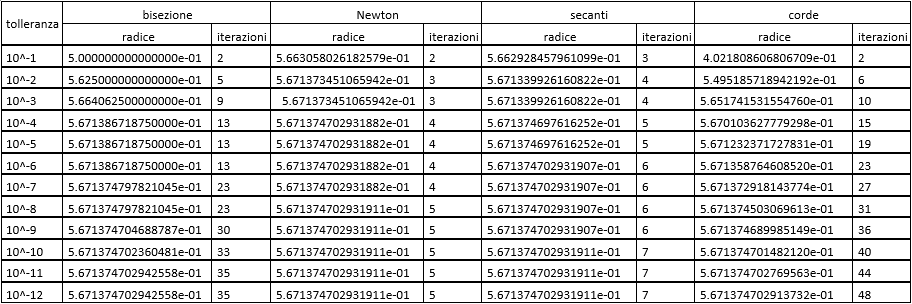
\includegraphics[width=1.3\textwidth]{img/tabella}
}
\\~\\
Nella tabella sono riportate le radici ricavate con ogni metodo e il relativo numero di iterazioni necessarie per ottenere tale risultato per ogni $tol = 10^{-i}, \quad i=1, 2,...,12$.\newline
Il metodo di bisezione e il metodo delle corde hanno una valutazione di funzione e convergenza lineare mentre il metodo di Newton ha due valutazioni di funzioni, una per la funzione e una per la sua derivata, e convergenza quadratica quindi col metodo di Newton si ha una maggiore velocit\'a nella ricerca della radice ma si ha anche un costo computazionale maggiore. Il metodo delle secanti ha una valutazione di funzione, quindi un costo computazionale minore del metodo di Newton,  e una convergenza $\approx$ 1.618, quindi ha una velocit\'a maggiore dei metodi di bisezione e delle secanti.